\documentclass[11pt]{article}

\usepackage[nohide,twocolumn]{ulecnot}
\usepackage{natbib}


\pagestyle{fancy}
\lhead{COGS 501 -- Formal Languages and Linguistics}
\chead{Finite Automata}
\rhead{Updated \it \today}
\lfoot{Umut \"Ozge}
\cfoot{}
\rfoot{Page \thepage/\pageref{LastPage}}
\setlength{\headheight}{13.6pt}

\newcommand{\emptystring}{\ensuremath{\epsilon}}

\usepackage{pgf}
\usepackage{tikz}
\usetikzlibrary{arrows,automata}
\tikzset{initial text={}}


\begin{document}


\section{Abstract machines}

\ezimeti{
\item Basic components of a computer: (i) central processing unit; (ii) memory;
(iii) input-output devices.
\item We are concerned with abstract machines, i.e.\ mathematical
descriptions of computing machinery.  

}

\section{Deterministic finite automata}

\ezimeti{
\item A \uterm{dfa} consists of a \uterm{reading head}, a \uterm{tape} and a
\uterm{finite control}.

\item The tape consists of squares which can hold a symbol.

\item The finite control consists of a set of finite states and an indicator
which shows the current state of the automaton.

\item The reading head starts at the leftmost position on the tape. The
automaton operates through discrete steps. At each step the reading head
advances one square right reading the symbol in its starting position, and
updating the state of the machine according to a \uterm{transition function}
which maps pairs of symbols and states to states.  

\begin{udefinition}[Deterministic finite automaton]
A dfa is a quintuple $\langle Q,\Sigma,\delta,q_0,F\rangle$ where
\ezimeti{
\item[]$Q$ is a set of \uterm{states}, 
\item[]$\Sigma$ is an \uterm{alphabet},
\item[]$q_0\in Q$ is the \uterm{initial state},
\item[]$F \subseteq Q$ is the set of \uterm{final states}.
}
and $\delta: Q\times\Sigma \mapsto Q$ is the \uterm{transition function}.
\end{udefinition}


\begin{uexercise}\label{extrace}
Take the fa $M= \langle\{q_0,q_1\},\{a,b\},\delta,q_0,\{q_0\}\rangle$ where 
$\delta$ is,
$$
\begin{array}{ccc}
q &\sigma&\delta(q,\sigma)\\ \hline
q_0 & a & q_0\\
q_0 & b & q_1\\
q_1 & a & q_1\\
q_1 & b & q_0
\end{array}
$$

Trace the processing of the string $aabba$ by $M$.
\end{uexercise}


\item Here are some formal definitions concerning the computations of fa:

\item[] As made clear by exercise \ref{extrace}, given any point during the
computation of an fa, the state the fa will end up when it runs out of input is
determined by the state at that point and the string yet to be read. 

\item[] Call $(q,w)$ a \uterm{configuration} of an fa $M$, where $q$ is the
current state and $w$ is the string on the tape including the current symbol and
what lies to the right of it.

\item[] For an fa $M=\langle Q,\Sigma,\delta,q_0,F\rangle$ the relation
\uterm{yields in one step}, defined over set of configurations and designated
with $\models_M$, is such that, 
$$
(q,w)\models_M(q',w') \text{ iff } w = \sigma w' \text{ for some }
\sigma\in\Sigma \text{ and } \delta(q,\sigma) = q'
$$

\item[] The relation \uterm{yields}, designated as $\models_M^*$, is the reflexive transitive closure of $\models_M$, 

\item[] An fa $M=\langle Q,\Sigma,\delta,q_0,F\rangle$  \uterm{accepts}
	a string $w\in\sigmastar$ iff $(q_0,w)\models_M^*(q_n,\epsilon)$ for some $q_n\in F$.  

\item The \uterm{language accepted} by $M$, designated $L(M)$ is the set of
strings accepted by $M$.

}
\section{State diagrams for fa}

\ezimeti{
\item  Finite automata can be conveniently represented by directed
graphs called \uterm{state diagrams}. Let's draw a state diagram for the
language accepted by the fa in Exercise \ref{extrace}.  


\begin{uexercise}\label{dfaex}
Draw the state diagrams of an accepting dfa for each language below:
\etaremune{
\item[\hyperlink{dfaex1}{1.}]
$\setabs{w\in\{a,b\}^*}{\text{each }a\text{ immediately
preceeded 
and immediately followed by } b}$.

\item[\hyperlink{dfaex2}{2.}]
$\setabs{w\in\{a,b\}^*}{w\text{ has } abab \text{ as a substring}}$.

\item[\hyperlink{dfaex3}{3.}]
$\setabs{w\in\{a,b\}^*}{w\text{ does not contain three consecutive }
b\text{'s}}$.

\item[\hyperlink{dfaex4}{4.}]
$\setabs{w\in\{a,b\}^*}{w\text{ has both } ab \text{ and } ba \text{ as
substrings}}$.

\item[\hyperlink{dfaex5}{5.}]
$\setabs{w\in\{a,b\}^*}{w\text{ has odd number of } a\text{'s and an even
number of } b\text{'s}}$.

\item[\hyperlink{dfaex6}{6.}]
$(ab \cup aba)^*$
}

\end{uexercise}

}
\section{Non-deterministic finite automata}

\ezimeti{

\item A \uterm{non-deterministic finite automaton} extends the notion of dfa in
the following respects:

\begin{itemize}
\item[i.] $\delta$ is no longer required to be a function;  
\item[ii.] \uterm{empty transitions} are allowed, i.e.\ the finite control is
allowed to advance the state without reading any symbol from the input tape;
\item[ii.] transitions are not limited to symbols, an nfa can read $w\in
\sigmastar$.
\end{itemize}


\begin{uexercise}
Provide an nfa for the languages 1, 2 and 6 of exercise \ref{dfaex}. 
\end{uexercise}


\item Finite automata $M_1$ and $M_2$ are \uterm{equivalent} if and only if
$L(M_1)=L(M_2)$.

\begin{utheorem}
For each non-deterministic finite automaton there exists an equivalent
deterministic finite automaton.
\end{utheorem}


\item There exists an algorithm to construct a dfa from a given nfa. The basic
logic of the algorithm is to treat \emph{sets} of states of the nfa as states of
the dfa. We will not study the algorithm in detail.

\begin{uexercise}
Provide nfa's that accept the following languages:
\begin{itemize}
\item[(a)] $(ab)^*(ba)^* \cup aa^*$
\item[(b)] $((ab \cup aab)^*a^*)^*$
\item[(c)] $((a^*b^*a^*)^*b)^*$
\item[(d)] $(ba \cup b^*) \cup (bb \cup a)^*$
\end{itemize}
\end{uexercise}
}

\section{Equivalence of FALs and regular languages}

\ezimeti{
\item We call a language $\mathcal{L}$ a \uterm{finite automaton language} (or fal), if
and only if there exists an fa $M$ such that $\mathcal{L} = L(M)$.
\item Finite automata and regular expressions are two alternative ways
of characterizing the same class of languages.
\begin{utheorem}[Kleene]
A set of strings is a finite automaton language if and only if it is a
regular language.
\end{utheorem}

\item We will prove by induction only the \emph{regular
expression-to-finite automaton}
side of the theorem:
	\ezimeti{
			\item We start by showing that the three basic regular expressions,
					$\emptyset$, $\epsilon$ and the unit language \textbf{a} for an
							arbitrary symbol $a$, have equivalent NFAs. 
			\item Then we show that finite automata are closed under
			union, concatenation and closure.
	}
}



\section{Properties of regular languages}

\ezimeti{
\item We have seen above that regular languages and FALs are closed
under the operations of union, concatenation and closure. Now we look at
intersection and complementation.

\item If a language $L \subseteq \Sigma^*$ is regular,\footnote{Note
the typo in Partee et al.\ p.\ 477, which says  $L \in \Sigma^*$
instead of $L \subseteq \Sigma^*$.}  then its complement, namely
$\Sigma^*-L$ is also regular. How can we prove this? (Hint: make use
of finite automata.)

\item From the above result, it follows that regular languages are
closed under intersection as well. Why? (Hint: DeMorgan!)


\item These properties can be used to decide whether a given language is regular
or not.

\begin{uexercise}
Is the language $L$ over $\{a,b\}$ whose strings has an even number of $a$'s and
odd length regular?
\end{uexercise}

}

% \ezimeti{
% \item Now we are ready to answer an important question: Is English -- or any
% other natural language -- a regular language?
% }

\section{A Way to determine that a language is not regular}

\ezimeti{
\item
Given a language $L$, we can sometimes tell that it is not a FAL (or a
regular language) by using a simple theorem.

\begin{utheorem}[Pumping Theorem for FALs]
If $L$ is an infinite FAL over an alphabet $\Sigma$, then there are
strings $x$,$y$,$z \in \Sigma$, such that  $y \not = \epsilon$ and
$xy^nz \in L$ for all $n \geq \mathrm{0}$.
\end{utheorem}

\begin{uexample}
Let us take a language that we know to be a FAL, namely \\ $\setabs{w \in
\crbr{a,b}^*}{\text{ $w$ has an odd number of $b$s}}$ and observe how the
Pumping Theorem applies.
\end{uexample}

\item Pumping Theorem can \emph{sometimes} be used to prove that a language
is not a FAL. 

\begin{uexercise}
Prove that $\setabs{w \in \{a,b\}^*}{w=a^nb^n \text{ for } n \geq 0}$ is not a FAL.
\end{uexercise}

% \begin{uexample}
% Prove that $\crbr{w \in \Sigma^*\ |\ w \text{ has equal number of $a$s
% and $b$s}}$ is not a FAL.
% \end{uexample}
}
% \section*{Self study}
% 
% To be updated\ldots
% 
% \cite{sudkamp97}, Chapter 6 up to Section 6.4 covers most of what we have seen
% so far. At certain points there are references to context-free grammars; ignore
% them for now. You may have difficulty in understanding some formal definitions
% in the book, concentrate on the examples.

\appendix
\section{Answers for selected exercises}
\begin{itemize}
\item[\ref{dfaex}] 
\begin{enumerate}
\hypertarget{dfaex1}{\item}


\fbox{\parbox[c]{0.41\textwidth}{\footnotesize
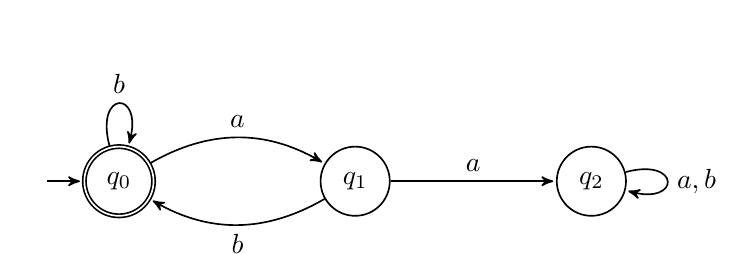
\begin{tikzpicture}[->,>=stealth',shorten >=1pt,auto,node distance=3.0cm,
                    semithick]
  \tikzstyle{every state}=[fill=none,draw=black,text=black]

  \node[initial,state,accepting] (0)                    {$q_0$};
  \node[state]         (1) [right of=0]	      {$q_1$};
  \node[state]         (2) [right of=1]	      {$q_2$};

  \path (0) edge [loop above]	node {$b$} 						(0)
  	    (0) edge [bend left]	node {$a$}				 		(1)
  	    (1) edge [bend left]	node {$b$}				 		(0)
  	    (2) edge [loop right]	node {$a,b$}				 		(2)
  	    (1) edge 				node {$a$}				 		(2);
\end{tikzpicture}
}
}

\hypertarget{dfaex2}{\item}

\fbox{\parbox[c]{0.41\textwidth}{\footnotesize
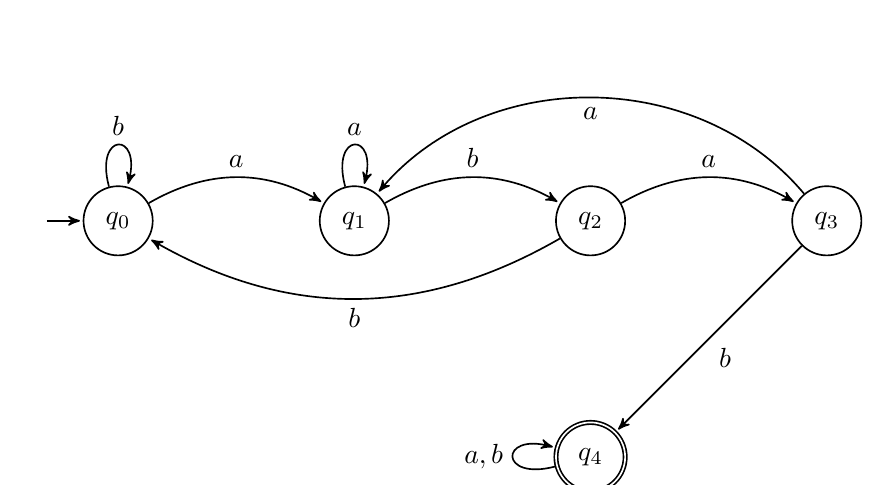
\begin{tikzpicture}[->,>=stealth',shorten >=1pt,auto,node distance=3.0cm,
                    semithick]
  \tikzstyle{every state}=[fill=none,draw=black,text=black]

  \node[initial,state] (0)                    {$q_0$};
  \node[state]         (1) [right of=0]	      {$q_1$};
  \node[state]         (2) [right of=1]	      {$q_2$};
  \node[state]         (3) [right of=2]	      {$q_3$};
  \node[state,accepting]         (4) [below of=2]	  {$q_4$};

  \path (0) edge [loop above]	node {$b$} 						(0)
  	    (0) edge [bend left]	node {$a$}				 		(1)
  	    (1) edge [loop above]	node {$a$}				 		(1)
  	    (1) edge [bend left]	node {$b$}				 		(2)
  	    (2) edge [bend left]	node {$a$}				 		(3)
  	    (2) edge [bend left]	node {$b$}				 		(0)
  	    (3) edge [bend right=50pt]	node {$a$}				 		(1)
  	    (4) edge [loop left]	node {$a,b$}				 	(4)
  	    (3) edge 				node {$b$}				 		(4);
\end{tikzpicture}
}
}

\hypertarget{dfaex3}{\item}

\fbox{\parbox[c]{0.41\textwidth}{\footnotesize
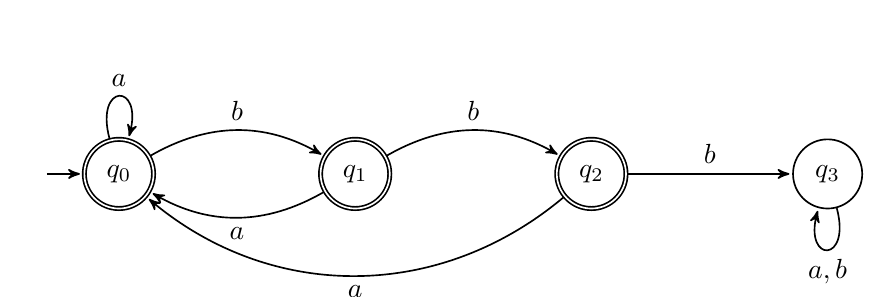
\begin{tikzpicture}[->,>=stealth',shorten >=1pt,auto,node distance=3.0cm,
                    semithick]
  \tikzstyle{every state}=[fill=none,draw=black,text=black]

  \node[initial,state,accepting]  (0)                    {$q_0$};
  \node[state,accepting]          (1) [right of=0]	      {$q_1$};
  \node[state,accepting]          (2) [right of=1]	      {$q_2$};
  \node[state]  		          (3) [right of=2]	      {$q_3$};

  \path (0) edge [loop above]	node {$a$} 						(0)
  	    (0) edge [bend left]	node {$b$}				 		(1)
  	    (1) edge [bend left]	node {$b$}				 		(2)
  	    (1) edge [bend left]	node {$a$}				 		(0)
  	    (2) edge            	node {$b$}				 		(3)
  	    (2) edge [bend left=40pt]	node {$a$}				 		(0)
  	    (3) edge [loop below]	node {$a,b$}				 	(1);
\end{tikzpicture}
}
}

\hypertarget{dfaex4}{\item}

\fbox{\parbox[c]{0.41\textwidth}{\footnotesize
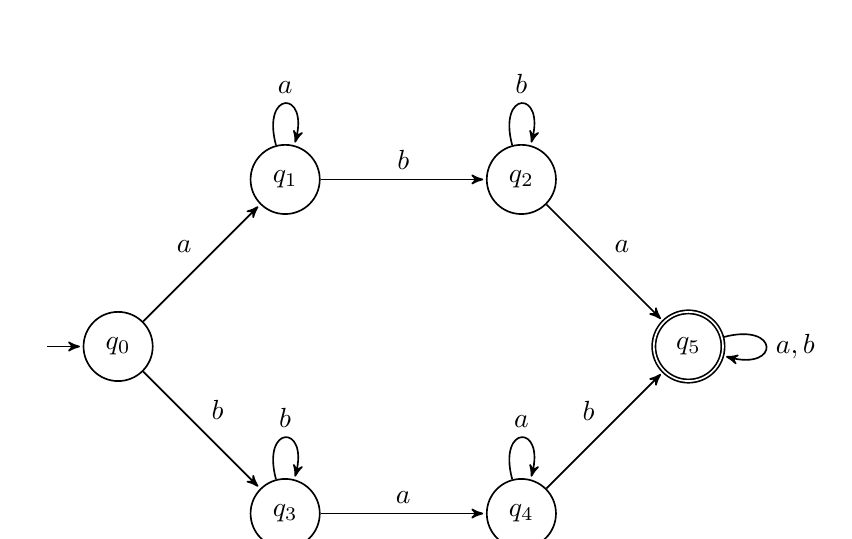
\begin{tikzpicture}[->,>=stealth',shorten >=1pt,auto,node distance=3.0cm,
                    semithick]
  \tikzstyle{every state}=[fill=none,draw=black,text=black]

  \node[initial,state]  (0)                       {$q_0$};
  \node[state]          (1) [above right of=0]	  {$q_1$};
  \node[state]          (2) [right of=1]	      {$q_2$};
  \node[state]          (3) [below right of=0]    {$q_3$};
  \node[state]          (4) [right of=3]	      {$q_4$};
  \node[state,accepting]          (5) [above right of=4]    {$q_5$};

  \path (0) edge			  	node {$a$} 						(1)
  	    (1) edge [loop above]	node {$a$}				 		(1)
  	    (1) edge 				node {$b$}				 		(2)
  	    (2) edge [loop above]	node {$b$}				 		(2)
  	    (0) edge 				node {$b$}				 		(3)
  	    (3) edge [loop above]	node {$b$}				 		(3)
  	    (3) edge  				node {$a$}				 		(4)
  	    (4) edge [loop above]	node {$a$}				 		(4)
  	    (4) edge 				node {$b$}				 		(5)
  	    (2) edge 				node {$a$}				 		(5)
  	    (5) edge [loop right]	node {$a,b$}				 		(5);
\end{tikzpicture}
}
}
\hypertarget{dfaex5}{\item}

\fbox{
\parbox[c]{0.41\textwidth}{

Let's agree on a simple convention: `ee' means the number of $a$'s and $b$'s are
both even; `oe' means odd number of $a$'s and even number of $b$'s; `eo' means
even $a$'s and odd $b$'s; `oo' means both are odd. These four situations exhaust
the logically possible states that a dfa can be in while processing a string of
$a$'s and $b$'s. We will construct our automaton on the basis of this
observation. We name our states according to our convention. Therefore the state
named `oe' -- odd $a$ even $b$ -- will be an accepting (=final) state.
\textbf{Please observe that the names we give to our states
is just to make the machine more understandable for humans. The names do not
mean anything to the machine. Any other naming would be equally good, provided
that the state transition function stays the same.}



\bigskip
{
\footnotesize

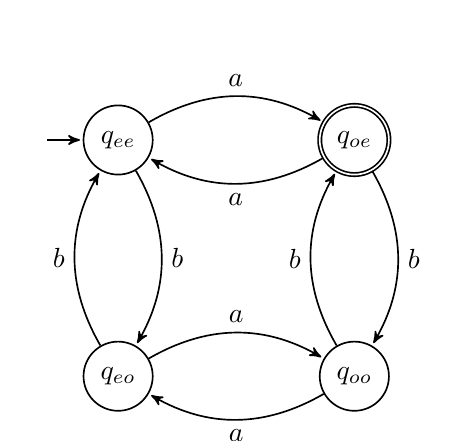
\begin{tikzpicture}[->,>=stealth',shorten >=1pt,auto,node distance=3.0cm,
                    semithick]
  \tikzstyle{every state}=[fill=none,draw=black,text=black]

  \node[initial,state]  (0)                       {$q_{ee}$};
  \node[state,accepting](1) [right of=0]	  {$q_{oe}$};
  \node[state]          (2) [below of=1]	      {$q_{oo}$};
  \node[state]          (3) [below of=0]    {$q_{eo}$};

  \path (0) edge	[bend left]	node {$a$}					(1)
  	    (1) edge	[bend left]	node {$a$}					(0)
  	    (1) edge 	[bend left]	node {$b$}				 	(2)
  	    (2) edge 	[bend left]	node {$b$}				 	(1)
  	    (2) edge 	[bend left]	node {$a$}				 	(3)
  	    (3) edge 	[bend left]	node {$a$}				 	(2)
	  	    (0) edge 	[bend left]	node {$b$}				 	(3)
  	    (3) edge 	[bend left]	node {$b$}				 	(0);
\end{tikzpicture}
}
}
}


\hypertarget{dfaex6}{\item}

\fbox{\parbox[c]{0.41\textwidth}{\footnotesize
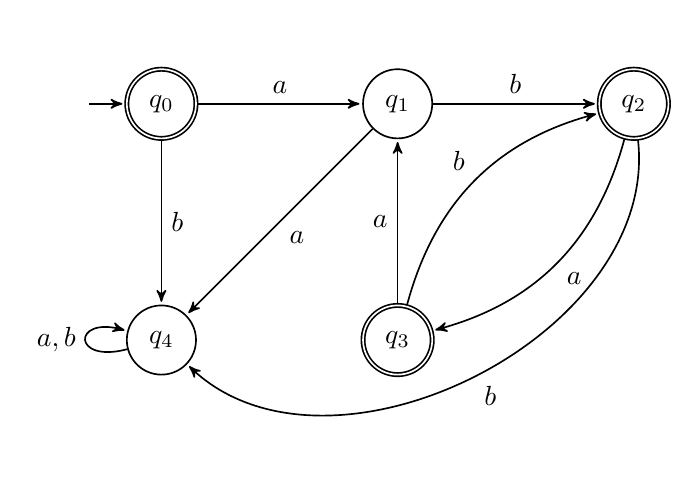
\begin{tikzpicture}[->,>=stealth',shorten >=1pt,auto,node distance=3.0cm,
                    semithick]
  \tikzstyle{every state}=[fill=none,draw=black,text=black]

	  \node[initial,state,accepting]  	(0)                    	{$q_0$};
  \node[state]          			(1) [right of=0]	  	{$q_1$};
	  \node[state,accepting]			(2) [right of=1]	   	{$q_2$};
	  \node[state,accepting]			(3) [below of=1]   		{$q_3$};
  \node[state]						(4) [below of=0]   		{$q_4$};

  \path (0) edge			  	node {$a$} 						(1);
  \path (0) edge			  	node {$b$} 						(4);
  \path (1) edge			  	node {$b$} 						(2);
  \path (1) edge			  	node {$a$} 						(4);
  \path (2) edge	[bend left]	node {$a$} 						(3);
  \path (2) edge	[bend left=70pt]	node {$b$} 						(4);
  \path (3) edge	[bend left]	node {$b$} 						(2);
  \path (3) edge				node {$a$} 						(1);
  \path (4) edge	[loop left]node {$a,b$} 					(4);

\end{tikzpicture}
}
}
\end{enumerate}
\end{itemize}

\bibliographystyle{natgig}
\bibliography{ozge}
\end{document}

\section{Conclusion}


